\documentclass{article}


\usepackage[english]{babel}
\usepackage{listings}

\usepackage[letterpaper,top=2cm,bottom=2cm,left=3cm,right=3cm,marginparwidth=1.75cm]{geometry}

% Useful packages
\usepackage{amsmath}
\usepackage{graphicx}
\usepackage[colorlinks=true, allcolors=blue]{hyperref}
\usepackage{listings}
\title{COSC 343: homework 1}
\author{Micah Sherry}

\begin{document}
\maketitle

\section{Floating Point System}

Assume that you are solving the quadratic equation $ ax^2 + bx + c = 0 $, 
with $ a = 1.22 $, $ b = 3.34 $, 
and $ c = 2.28 $, using a normalized floating-point system with base = 10, $ p = 3 $ 
(the mantissa has only three digits). That is all numbers in the system are of the form:
$$ (0.d_1d_2d_3)_{10} \times 10^{\pm k}$$
where $d1 \neq 0$ 
    \begin{enumerate}
        \item What is the computed value of the discriminant $ b^2- 4ac$? 
        \\ The first step I took was to find $b^2$ in this floating point system for that I got $b^2 = .111 \times 10^2$. The next step I took was to calculate $ a \times c$ and for that I got $ a \times c = .270 \times 10^1$. Then I multiplied that value by 4 to get $ 4\times a \times c = .108 \times 10^2 $. Finally putting everything together I got $b^2 - 4\times a \times c = .300\times 10^{-2}$
        \item What is the exact value of the discriminant in real (exact) arithmetic?
        \\ The exact value for the discriminate $ \approx .0292 $
        \item What is the relative error in the computed value of the discriminant?
        \\ The relative error is calculated with $$ \frac{|true - approx|}{|true|}$$ using this formula I got $$\frac{|0.0292 - 0.003|}{|0.0292|}= 0.897$$
    \end{enumerate}

\section{The harmonic series}
The harmonic series is known to diverge to $\infty$. The nth partial sum approaches $\infty$ at the same rate as ln(n). Euler’s constant is defined to be
$$\gamma = \lim_{n \to \infty } \left( \sum_{k=1}^{n}\frac{1}{k} - ln(n) \right)\approx 0.57721$$
\begin{enumerate}
	
    \item If your computer ran a program for a week based on the pseudo code:
    \begin{lstlisting}
    	x = 1.0;
    	s = 1.0;
    	repeat
    		x = x + 1.0;
    		s = s + 1.0/x;
    	end repeat
    \end{lstlisting}
   what is the largest value of s it would obtain? 
    \\Let $\epsilon_{mach} $ denote the machine precision.   $$\epsilon_{mach} \approx 10^{-16}$$ 
    What this tells us is that the loop used to calculate the harmonic series will stop being accurate if  $$ \frac{1}{n} < \epsilon_{mach}$$ where n is the number of iterations of the loop. 
    using algebra we find that the $$\frac{1}{\epsilon_{mach}} < n$$ meaning that using this loop the harmonic series will stop being accurate after the $10^{16}th$ iteration of the loop. To find the max value of the nth partial sum I will use the fact that 
    $$0.57721+ln(n)\approx \sum_{k=1}^{n}\frac{1}{k}$$
    Then substituting $10^{16}$ in for n we can find the maximum value of the harmonic series we can compute using this method is $$s \approx 37.42$$
    \item Write and test a program that uses a loop of at least 5000 steps to estimate Euler’s constant and Make a plot of the values
    \begin{figure}[hbt!]
        \centering
        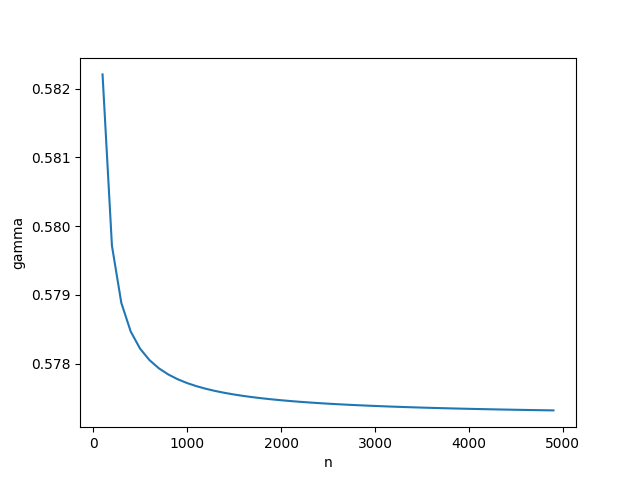
\includegraphics[width=.75\linewidth]{gamma.png}
        \caption{ gamma  approximation}
        \label{fig: gamma  approximation}
    \end{figure}
    
\end{enumerate}
 
\pagebreak
\section{Finite Difference}
 Write a program to compute an approximate value for the derivative of a function
using the finite-difference formula.
$$ f^{\prime}(x) \approx \frac{f(x+h)-f(x)}{h}$$
Test your program using the function tan(x) for x = 1. Determine the error by
comparing it with the square of the built-in function sec(x). 
for the magnitude of the error.
    \begin{figure}[hbt!]
        \centering
        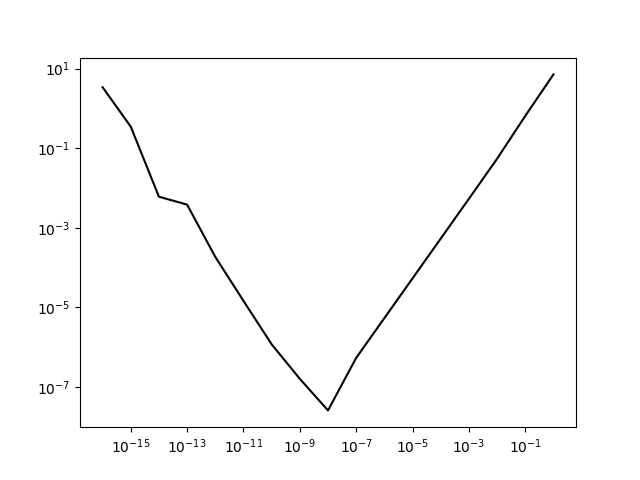
\includegraphics[width=.75\linewidth]{finite_diff.png}
        \caption{ finite difference}
        \label{fig: finite diffrence}
    \end{figure}
    

    \begin{enumerate}
        \item Is there a minimum value for the magnitude of the error?
        \\ There is a local minimum at the $ h \approx 10^{-8} $.   the value of the minimum error $\approx 2 \times 10^{-8}$
        \item How does the corresponding value for h compare with the value $ h \approx \sqrt{\epsilon_{mach}}$ where $\epsilon_{mach} \approx 10^{-16}$ is the machine precision value found in class examples? \\
        the value of h where there is a minimum is the square root of is $\epsilon_{mach}$. I suspect that the minimum in at this value is related to the fact that $$\frac{d}{dx}tan(x)=sec^{2}(x)$$. However I am unsure how to confirm of deny that hypothesis.  
        \item Repeat the exercise using the centered difference approximation.
        $$ f^{\prime}(x) \approx \frac{f(x+h)-f(x-h)}{2h}$$
        \pagebreak
        \begin{figure}[hbt!]
        	\centering
        	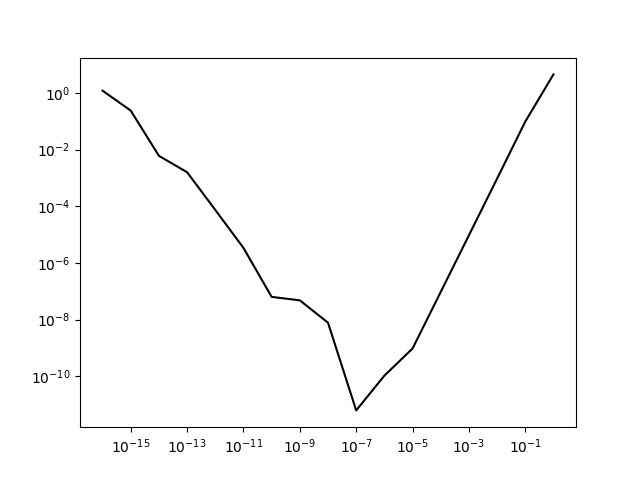
\includegraphics[width=.75\linewidth]{finite_diff2png.png}
        	\caption{ symmetric finite difference}
        	\label{fig: symmetric finite diffrence}
    	\end{figure}
        \\ Using this formula the error reaches a minimum faster it reaches a minimum at $ h \approx 10^{-7} $. The value of the minimum error $\approx 6 \times 10^{-12} $. This part confused me at first because the error is several orders of magnitude smaller than first finite difference formula's error. My first assumption was that these to methods would be very similar to each other. To see the reason why this occurs I started plotting the secant lines associated with each of these formulas.
        \begin{figure}[hb!t!]
        	\centering
        	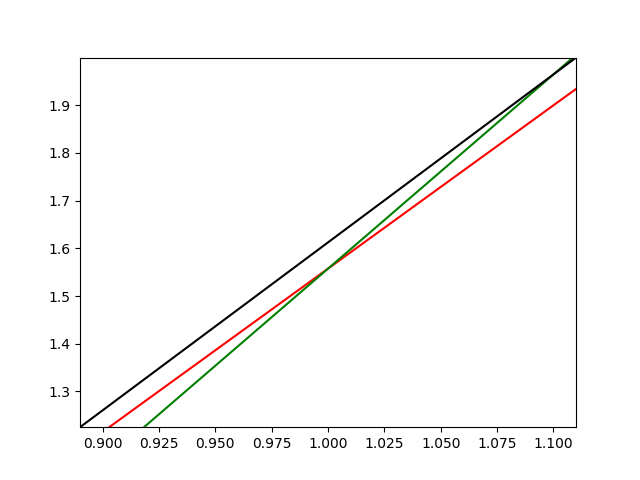
\includegraphics[width=.75\linewidth]{tangent_to_tan.png}
        	\caption{secant lines}
        	\label{fig: secant lines}
        \end{figure} 
        \\The red line is the line tangent to tan(x) at x = 1
        \\The black line is formed by the points (x-h, tan(x-h)) and (x+h, tan(x+h))
        \\The green line is formed by the points (x, tan(x)) and (x+h, tan(x+h))
        \\Notes: the tan(x) is not graphed because it made the diagram harder to veiw, $x = 1 $ and $ h = 0.1$ for this graph. 
        \\ What does this graph tell us? The red line represent the true slope of the tangent line. Lines that are closer to parallel (to the red line) approximate the slope of the tangent better. So this visually explains why we see smaller errors while using the symmetric difference formula. To see why the symmetric difference formula is better. you can use the Mean Value Theorem to show that the Symmetric difference formula guarantees that there is a point on the interval (x-h, x+h) that is tangent to the curve at x and then use Mean Value theorem  to see that the finite difference formula does not guarantee that there is a point on the interval (x, x+h) that is tangent to the curve at x. 
    
    \end{enumerate}



\end{document}